\section{Comparison between the Designs}\label{sec:comparison}
The two designs can now be analyze and together, to compare their performance.

In \autoref{fig:xbdot_comp} and \ref{fig:yaw_comp} a similar simulation than in the previous cases can be seen.
\begin{figure}[H]
    \captionbox 
    {   
        Comparison of the response of both controllers in $x_\mathrm{b}$, when a disturbance is applied (at 3 s) and when a reference is set in yaw (at 10 s).
        \label{fig:xbdot_comp}
    }                                                                 
    {                                                                  
        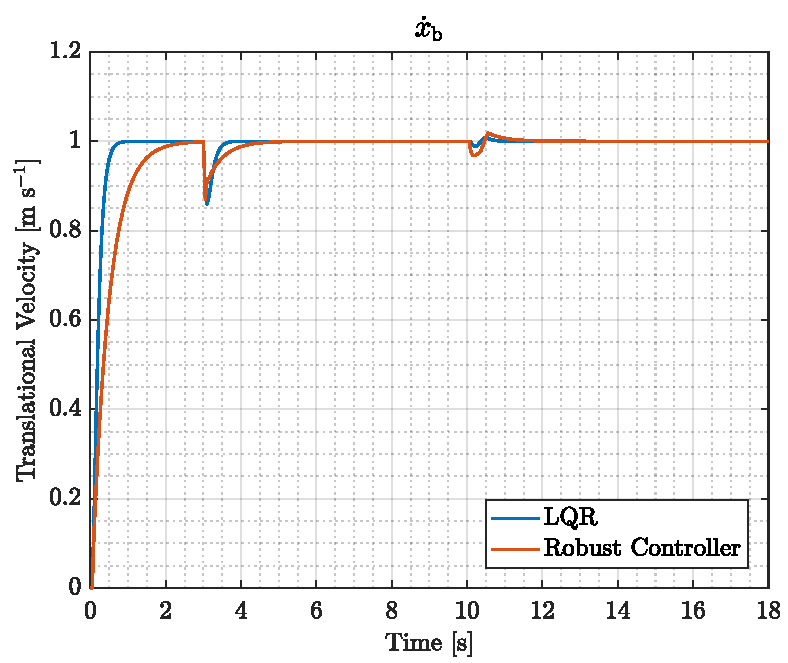
\includegraphics[width=.45\textwidth]{figures/xbdot_comp}         
    }                                                                    
    \hspace{5pt}                                                          
    \captionbox  
    {      
        Comparison of the response of both controllers in $\psi$.
        \label{fig:yaw_comp}
    }                                                                          
    {
        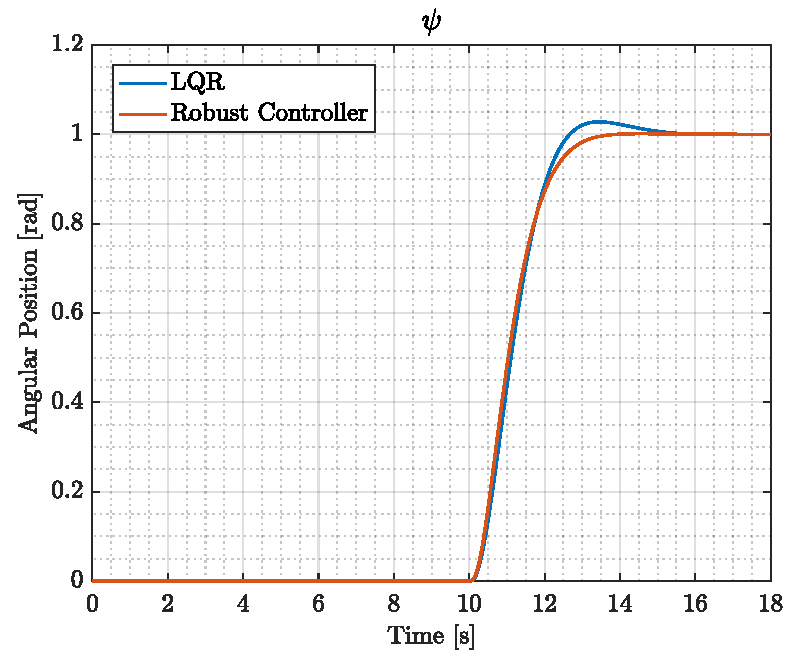
\includegraphics[width=.45\textwidth]{figures/yaw_comp}
    }
\end{figure}

The simulation in this case includes a step disturbance at 3 s in the form of wind force to analyze how both controllers can handle this situation.

\fxnote{Finish description with final graphs and check seconds and settling times with final graphs in the comparison.}